\documentclass{article}

% Recommended packages
\usepackage{microtype}
\usepackage{graphicx}
\usepackage{subfig}
\usepackage{booktabs}
\usepackage{hyperref}
% xelatex font setup — use system fonts so the ICML times/helvetica/courier
% requests in icml2025.sty resolve cleanly without the Type1 .tfm files.
\usepackage{fontspec}
\IfFontExistsTF{Times New Roman}{\setmainfont{Times New Roman}}{}
\IfFontExistsTF{Helvetica}{\setsansfont{Helvetica}}{}
\IfFontExistsTF{Courier New}{\setmonofont{Courier New}}{}
% multirow not used; cleveref unavailable on this TeX install — minimal shim follows.
\makeatletter
\providecommand{\Cref}[1]{%
  \def\@cref@@@{#1}%
  \edef\@cref@prefix{\expandafter\@cref@parse@\@cref@@@:\@nil}%
  \@cref@printprefix{\@cref@prefix}~\ref{#1}}
\def\@cref@parse@#1:#2\@nil{#1}
\def\@cref@printprefix#1{%
  \ifcsname @cref@prefix@#1\endcsname
    \csname @cref@prefix@#1\endcsname
  \else Sec\fi}
\@namedef{@cref@prefix@fig}{Figure}
\@namedef{@cref@prefix@tab}{Table}
\@namedef{@cref@prefix@sec}{Section}
\@namedef{@cref@prefix@eq}{Eq.}
\providecommand{\cref}[1]{\Cref{#1}}
\makeatother

\newcommand{\theHalgorithm}{\arabic{algorithm}}

\usepackage[accepted]{icml2025}

\usepackage{amsmath}
\usepackage{amssymb}
\usepackage{mathtools}
\usepackage{amsthm}
% cleveref shimmed above

\icmltitlerunning{HW11: Layer-wise Analysis of VLM Features}

\begin{document}

\twocolumn[
\icmltitle{Layer-wise Analysis of Internal VLM Features \\
           via Logit Lens on Qwen2-VL-2B-Instruct}

\begin{center}
    \textbf{Ivan A. Novosad} \\
    \texttt{inovosad@hse.ru} \\
\end{center}

\vskip 0.3in
]

% ===================================================================
\section{Introduction}
\label{sec:intro}

I ran the logit lens on \textbf{Qwen2-VL-2B-Instruct} across five feature categories---color, shape, counting, spatial relations, and attribute-object binding---on 1250 controlled synthetic images.
Color, shape, and compositional binding all share a sharp two-layer transition at L22$\to$L23 rather than a gradual rise; binding shows up one layer after unbound color, with the distractor color already pinned near zero.
Counting falls apart for $n\ge4$---the model floors at ``three''---and even count ``one'' has to fight a plural prior until L27.
``Below'' is the strangest case: P(below) rises through L24, then \emph{decays}, and every L28 error produces ``right.''
\citet{neo2025interpreting} previously reported best object-identity decoding around layer~25 of 28 on this same backbone; this paper extends the per-layer breakdown to the four other feature classes.

% ===================================================================
\section{Method}
\label{sec:method}

\subsection{Model}

Qwen2-VL-2B-Instruct: 28 decoder layers, hidden size 1536, pre-norm RMSNorm, fp16 on a T4.
The lens is well-defined:
\begin{equation}
    p_\ell = \text{softmax}\!\left(W_U \cdot \text{RMSNorm}(h_\ell)\right)
    \label{eq:logitlens}
\end{equation}
$h_\ell$ is the residual-stream hidden state at layer~$\ell$ and $W_U$ is the unembedding matrix.

\subsection{Features and Dataset}

Five synthetic datasets, all 448$\times$448 px on a light gray (\texttt{\#D0D0D0}) background, reproducible per-image seeds.

\paragraph{Color (200 images).} A single circle ($r{=}60$\,px) in one of four colors (red, blue, green, yellow), centered with $\pm30$\,px jitter.

\paragraph{Shape (200 images).} Four shapes (circle, square, triangle, 5-pointed star), white fill with black outline, jittered around center.
Color held constant.

\paragraph{Counting (250 images).} $N \in \{1,\ldots,5\}$ red circles ($r{=}25$\,px) at random non-overlapping positions.

\paragraph{Spatial relations (200 images).} A red circle and a blue square in four configurations (left, right, above, below).
Positions are axis-aligned so the only signal differentiating ``above'' from ``below'' is the vertical coordinate---an earlier non-aligned version gave the model a horizontal cue and confused it.

\paragraph{Attribute-object binding (400 images).} Contrastive pairs.
Image~A: red circle on the left, blue square on the right; image~B swaps the colors.
The question ``What color is the circle?'' should produce ``red'' for A and ``blue'' for B.
200 pairs test whether the model binds color to the queried object or just registers ``red'' and ``blue'' both being present.

\subsection{Prompt Design}

Every prompt prefills the assistant turn so the answer lands at a known token position.
Color, for example:
\begin{quote}
\small
\texttt{USER: <image> What color is the object? Answer with one word.} \\
\texttt{ASSISTANT: The color is}
\end{quote}
The model's next token after ``is'' is the answer.
Every target word has a single-token surface form in the Qwen2 tokenizer ($V{=}151{,}936$).

For counting, digit prompts give ``\texttt{ 4}''---a space token followed by the digit---useless for a single-position lens, so I switched to word-form targets (``one'' through ``five''), each one token.
For spatial relations, the only template (out of six I tried) that reliably gave a single-word completion was ``Is the red circle above, below, left of, or right of the blue square? Answer with one word.'' with prefill ``Answer:''.

\subsection{Metrics}

At the answer position---last token of the prefill---and at each of the 29 hidden states (embedding + 28 layers) I record P(target) summed over single-token surface-form IDs, margin (P(target) $-$ $\max_j$ P(distractor$_j$) across the other classes), rank, and full-vocabulary entropy.
Aggregates use bootstrap 95\% CIs (1000 resamples).

% ===================================================================
\section{Results}
\label{sec:results}

The full sweep is 1250~images $\times$ 29~layers $=$ 36{,}250~measurements.

\subsection{Phase Transition at L22--L23}

\Cref{fig:heatmap} plots mean P(target) across every layer and class.
There's a hard boundary at L22--L23: below it, nothing is decodable; above it, every working feature is already strong.
The transition takes 2--3 residual blocks, not a smooth ramp.
\Cref{tab:emergence} has the numbers.
For color, P(target) goes from 0.001 at L22 to 0.413 (95\% CI [0.391, 0.437]) at L23---a 400$\times$ jump in one layer.
Shape and binding hit the same window.

\begin{figure}[t]
    \centering
    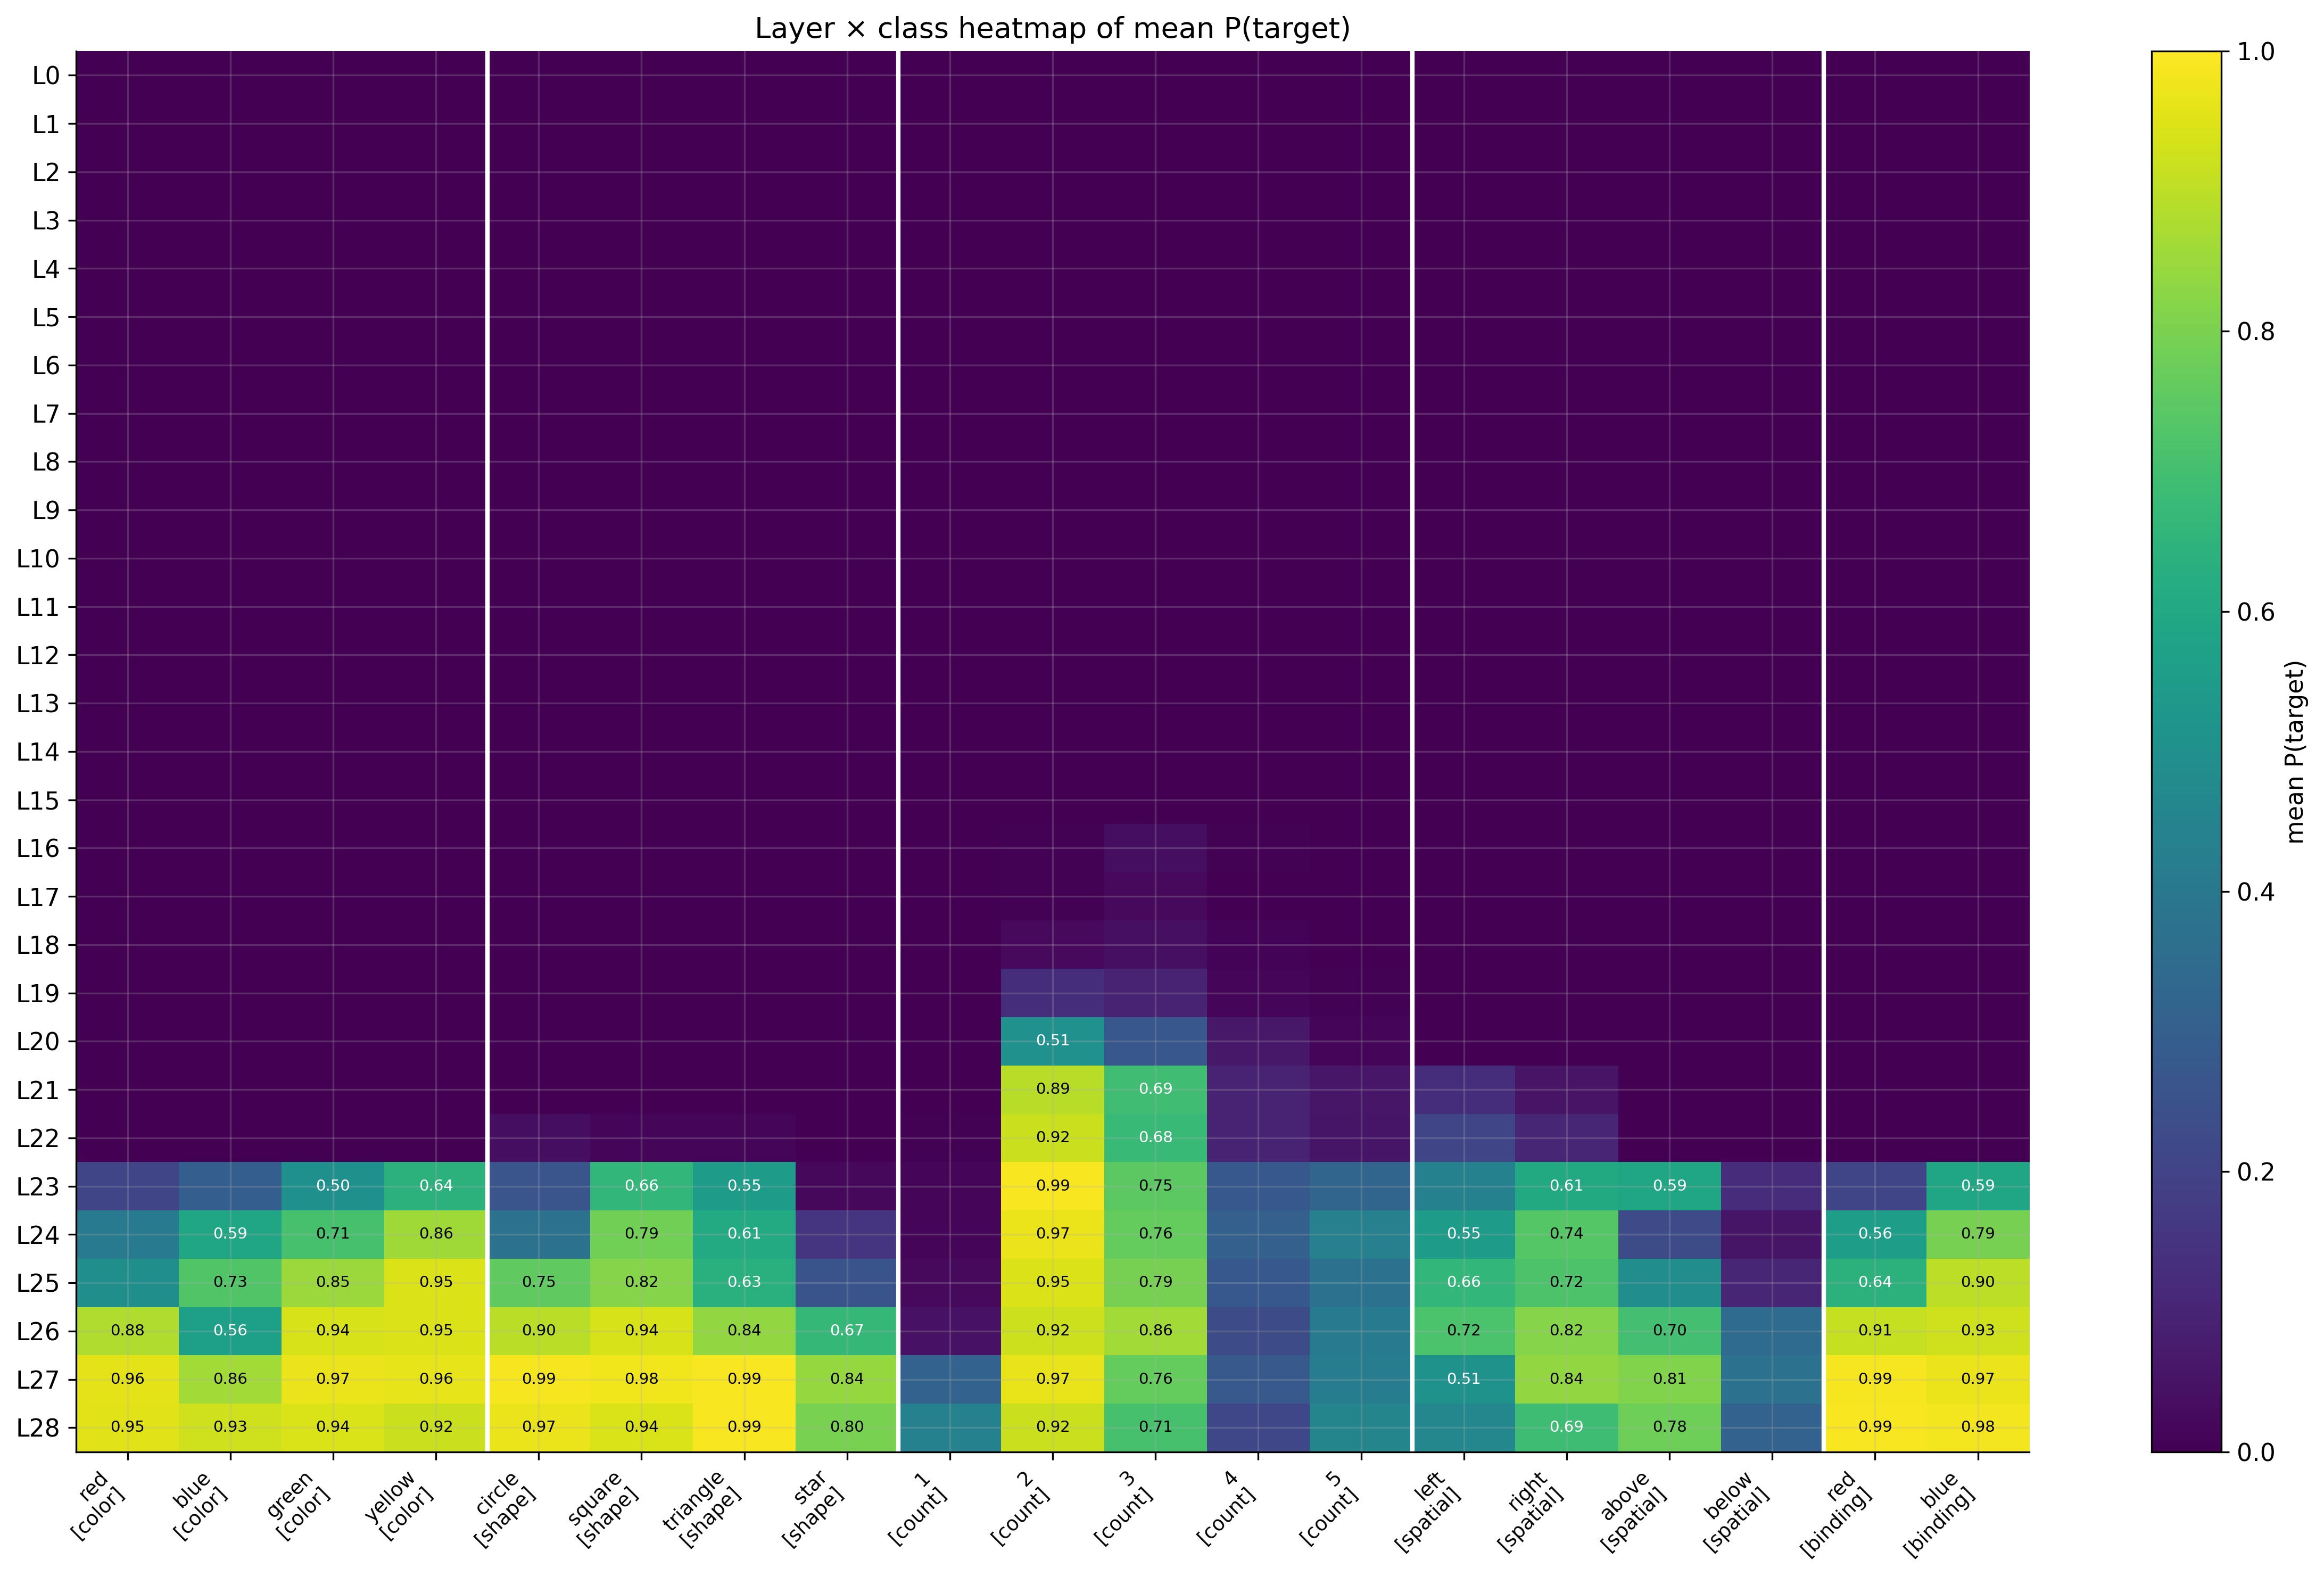
\includegraphics[width=\columnwidth]{fig2_heatmap.png}
    \caption{Layer $\times$ class heatmap of mean P(target). Cells with value $>0.5$ are annotated. The L23 boundary cleanly separates zero signal from strong feature decoding for every working class. The ``below'' column and the count ``one''/``four'' columns stay dark across all 29 rows.}
    \label{fig:heatmap}
\end{figure}

\begin{table}[t]
\centering
\small
\caption{Feature emergence: mean P(target) at key layers and L28 accuracy (rank$_\text{target}{=}0$). Emergence layer = first layer with mean P(target)$>$0.1.}
\label{tab:emergence}
\begin{tabular}{lccccc}
\toprule
\textbf{Category} & \textbf{L21} & \textbf{L23} & \textbf{L25} & \textbf{L28} & \textbf{Acc.} \\
\midrule
Color   & 0.000 & 0.413 & 0.755 & 0.936 & 100\% \\
Shape   & 0.001 & 0.374 & 0.617 & 0.925 & 100\% \\
Binding & 0.000 & 0.400$^\dagger$ & 0.770$^\dagger$ & 0.987 & 100\% \\
Count   & 0.349 & 0.522 & 0.484 & 0.548 & 71\% \\
Spatial & 0.046 & 0.307 & 0.473 & 0.562 & 78\% \\
\bottomrule
\end{tabular}
\vspace{2pt}
{\footnotesize $^\dagger$Binding values are margin (P(target)$-$P(distractor)), not raw P(target).}
\end{table}

\begin{figure*}[t]
    \centering
    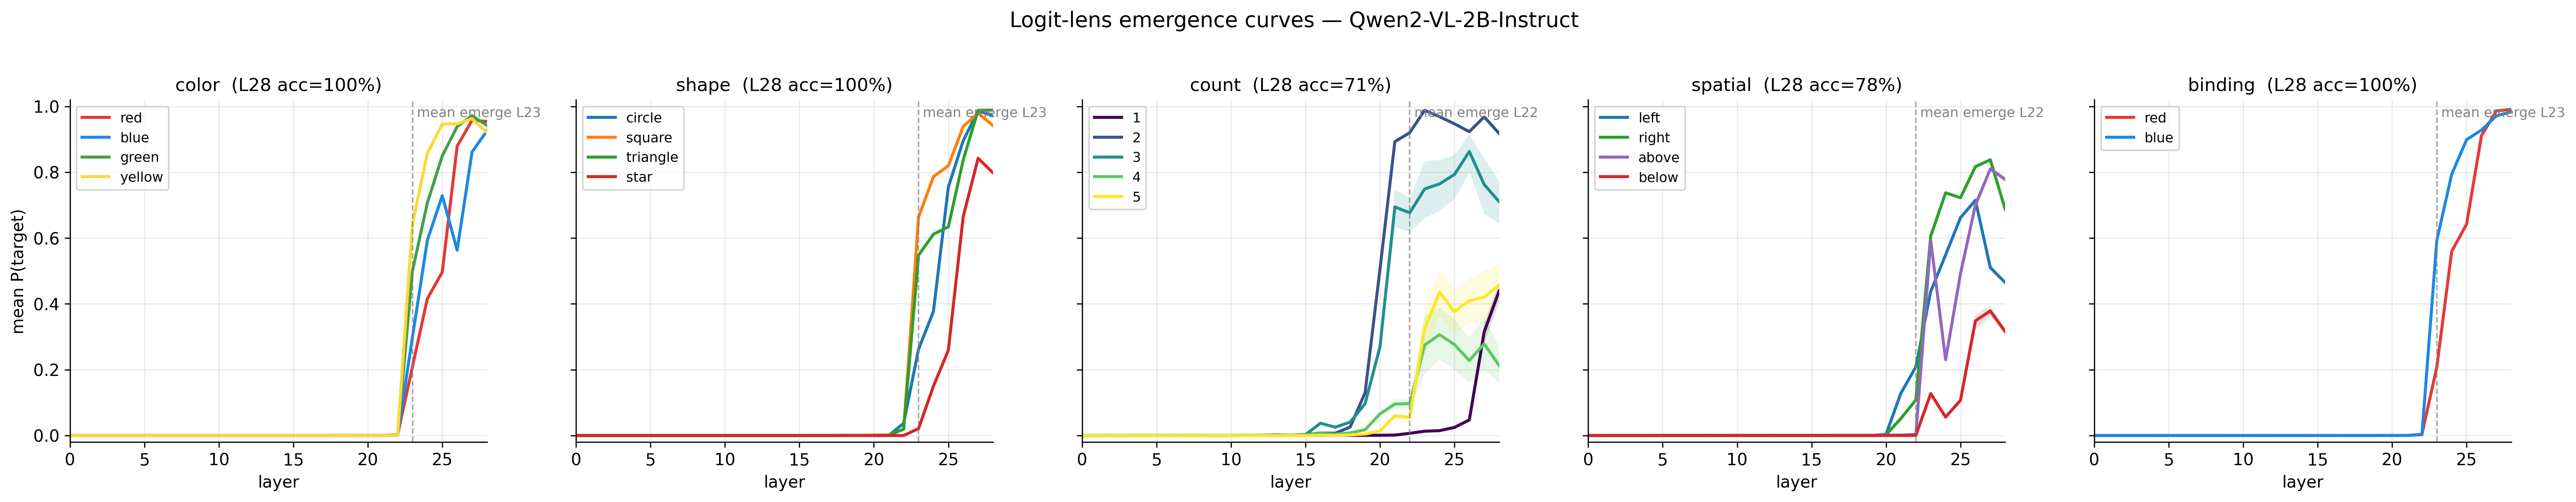
\includegraphics[width=\textwidth]{fig1_emergence_curves.png}
    \caption{Logit-lens curves: mean P(target) vs.\ layer for the five categories, broken out by class. Dashed vertical lines mark the per-category emergence threshold (mean P~$>$~0.1). Color and shape share the same sharp L23 transition; counting splits, with ``two'' at L19 and ``one'' not appearing until L27; ``below'' never settles; binding differentiates A vs.\ B from L23.}
    \label{fig:emergence}
\end{figure*}

\subsection{Color and Shape}

Color and shape are the cleanest features.
All four colors emerge together at L23 (P$>$0.2 each, no privileged hue---\Cref{fig:emergence}, leftmost panel), and by L26 every one is rank-0 with P$>$0.88.
At L28, per-class accuracy is 100\% across the board; red sits highest at P$=$0.955, yellow lowest at P$=$0.921, and the gap is well within the bootstrap CI.

Shape works on the same schedule with one small lag---the 5-pointed star arrives a layer late (L24 vs.\ L23 for circle, square, triangle) and plateaus at P$=$0.798 instead of the 0.94--0.99 the other three reach.
My guess is the white-on-gray star activates a thinner visual prior than the solid filled shapes, but the lens alone can't prove that.

\subsection{Binding: Compositional, Not Bag-of-Words}

The binding test is whether the model attaches ``red'' to ``circle'' (compositional) or just registers that both ``red'' and ``circle'' apply somewhere in the image (bag-of-words).
On this dataset the answer is compositional---\Cref{fig:binding}.

Panel~(b) is the one to look at: P(distractor) stays below 0.01 at \emph{every} layer.
The model never goes through a phase of ``I see red but I don't know whether it belongs to the circle or the square.''
When the signal first appears, it's already bound.
Panel~(d) is the harder check---pair-level accuracy (both A and B correct on the same pair) is exactly 0\% through L23 and 100\% from L24, which kills the ``the model just always says one color'' explanation.
You can't get 100\%/100\% single-side accuracy on both A and B by predicting the same color twice.

Binding emerges one layer after unbound color (L24 vs.\ L23).
Whether that one-layer gap is a real compositional circuit or just later softmax sharpening, the lens can't tell---you'd need patching or activation ablation.

\begin{figure}[t]
    \centering
    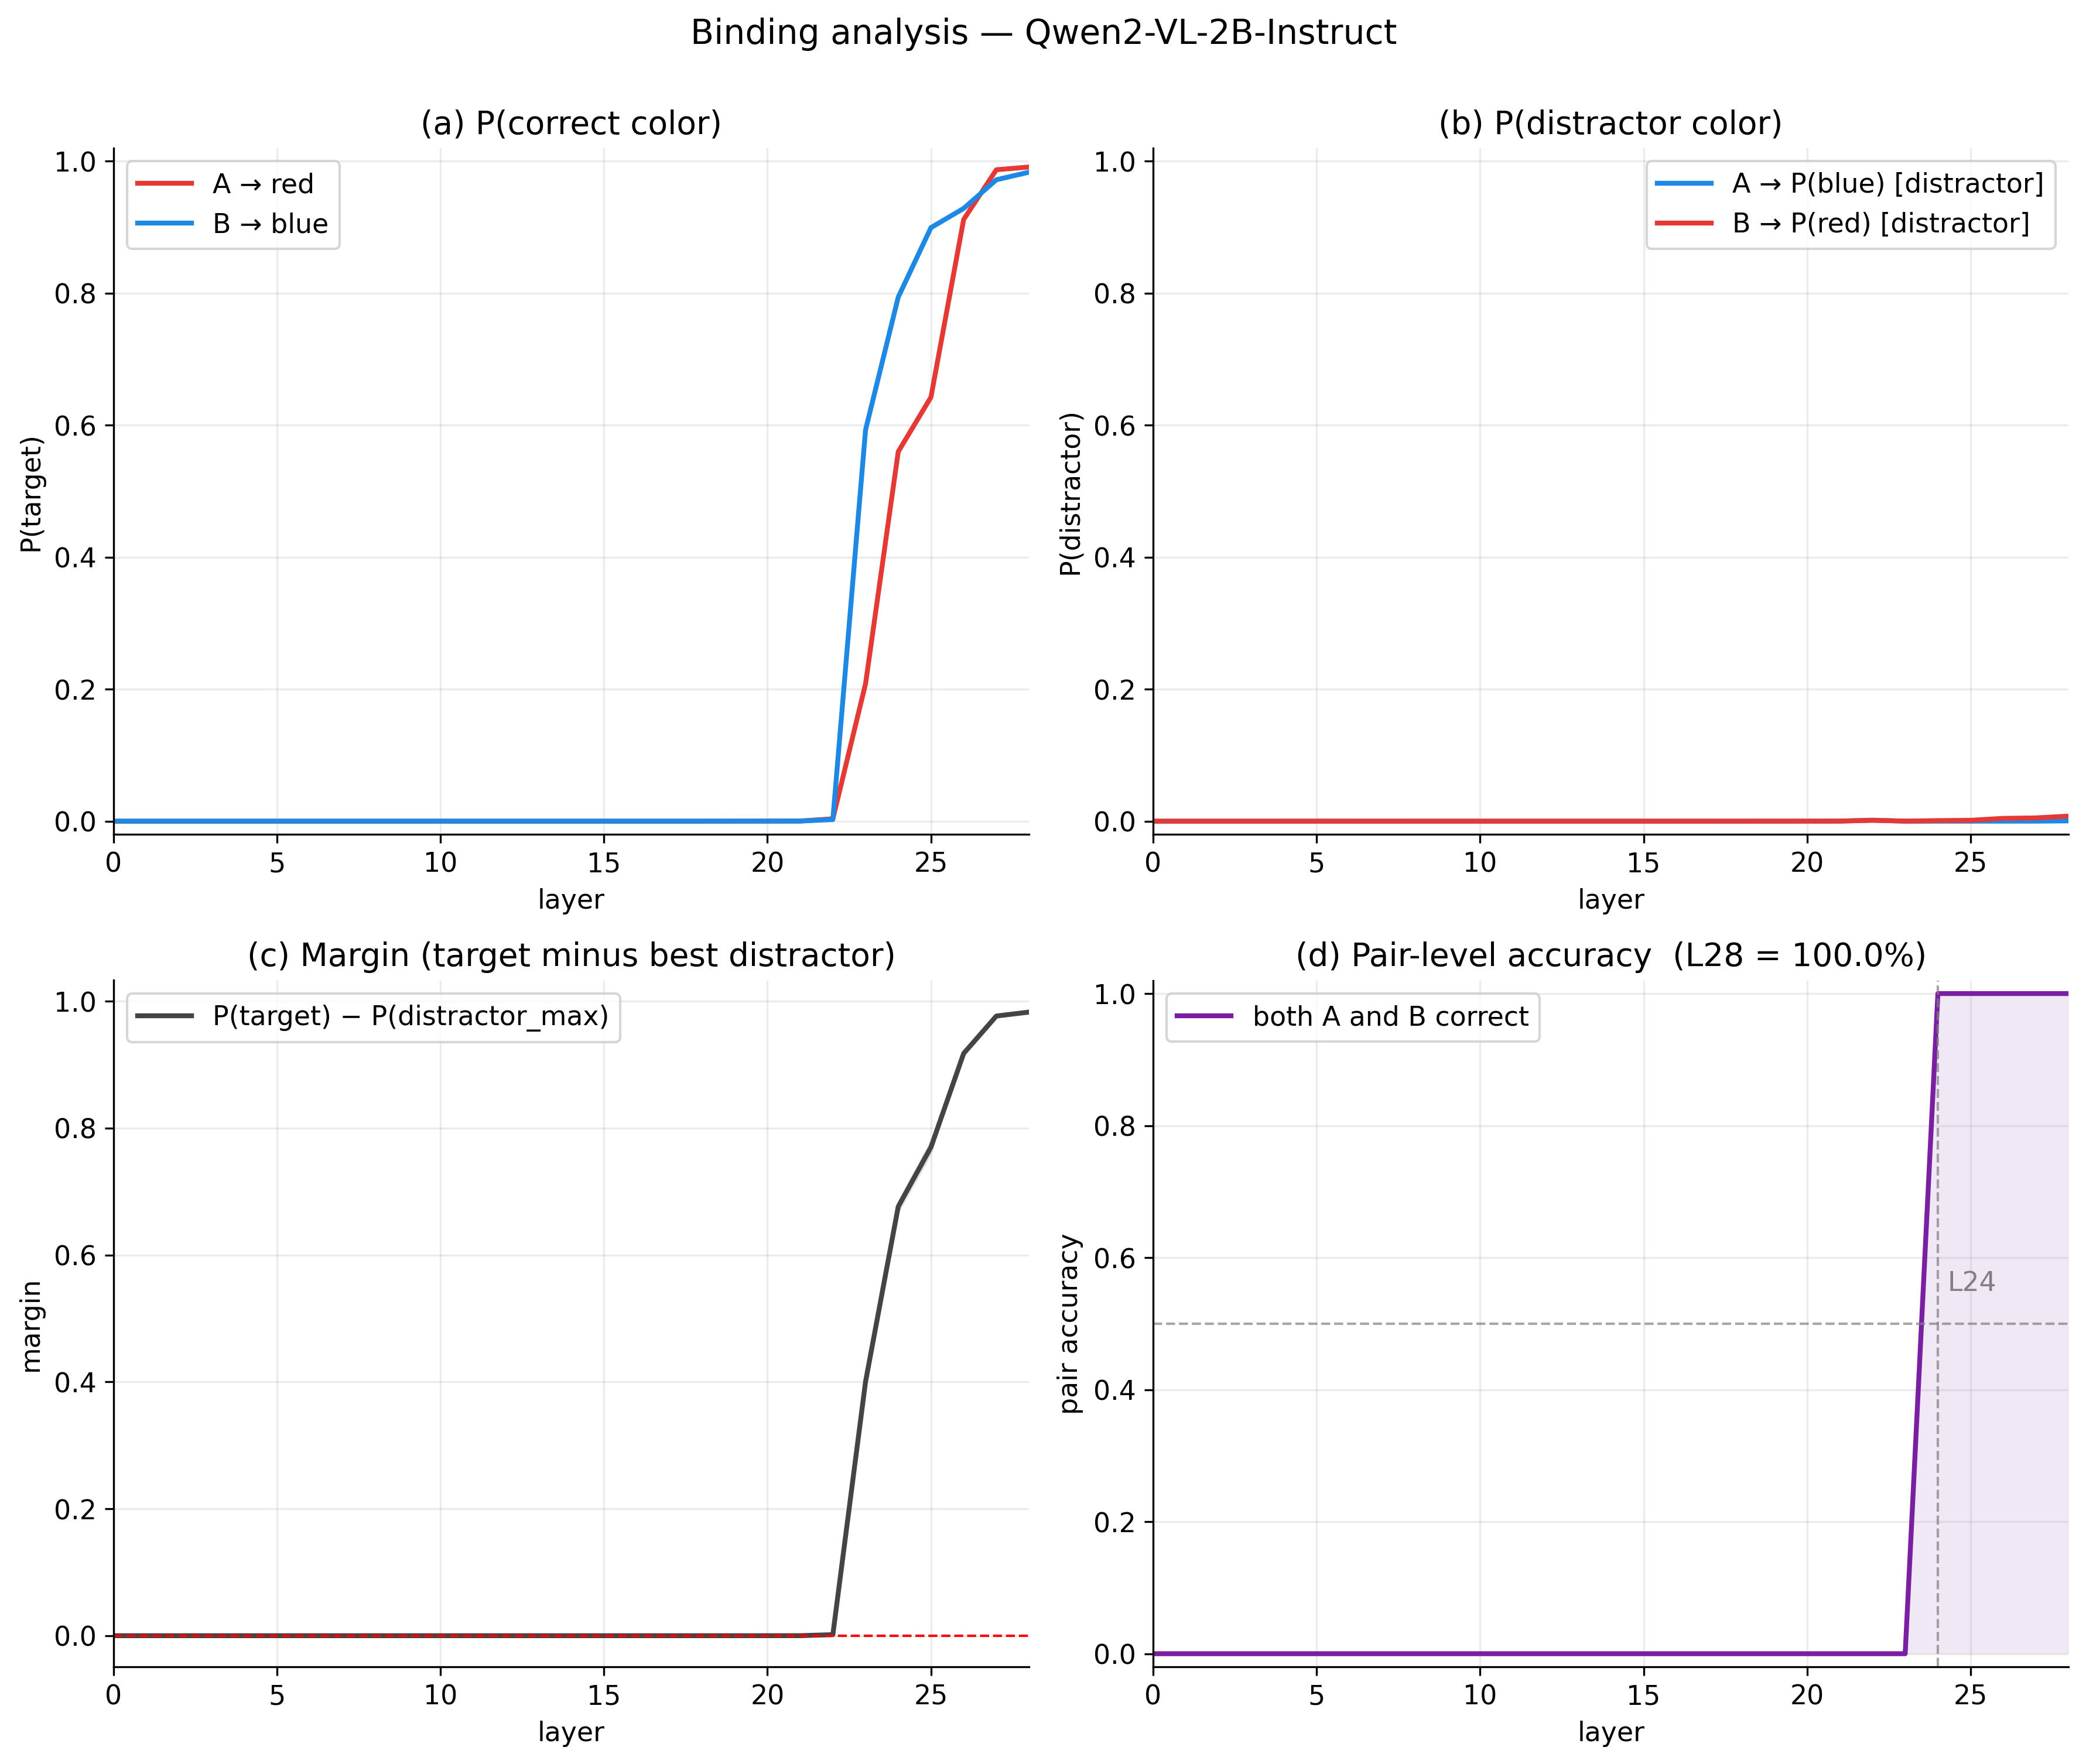
\includegraphics[width=\columnwidth]{fig3_binding.png}
    \caption{Binding analysis. (a)~P(correct color) for A$\to$red and B$\to$blue. (b)~P(distractor color)---stays at zero throughout, killing the bag-of-words alternative. (c)~Margin (target minus distractor). (d)~Pair-level accuracy: 0\% through L23, 100\% from L24.}
    \label{fig:binding}
\end{figure}

\subsection{Counting: Subitizing Ceiling at Three}

Counting is the first feature that doesn't work.
\Cref{fig:count} splits cleanly: ``two'' and ``three'' saturate by L21--L23 (P$>$0.85), while ``four'' and ``five'' plateau at 0.2--0.45 and never recover.

\begin{figure}[t]
    \centering
    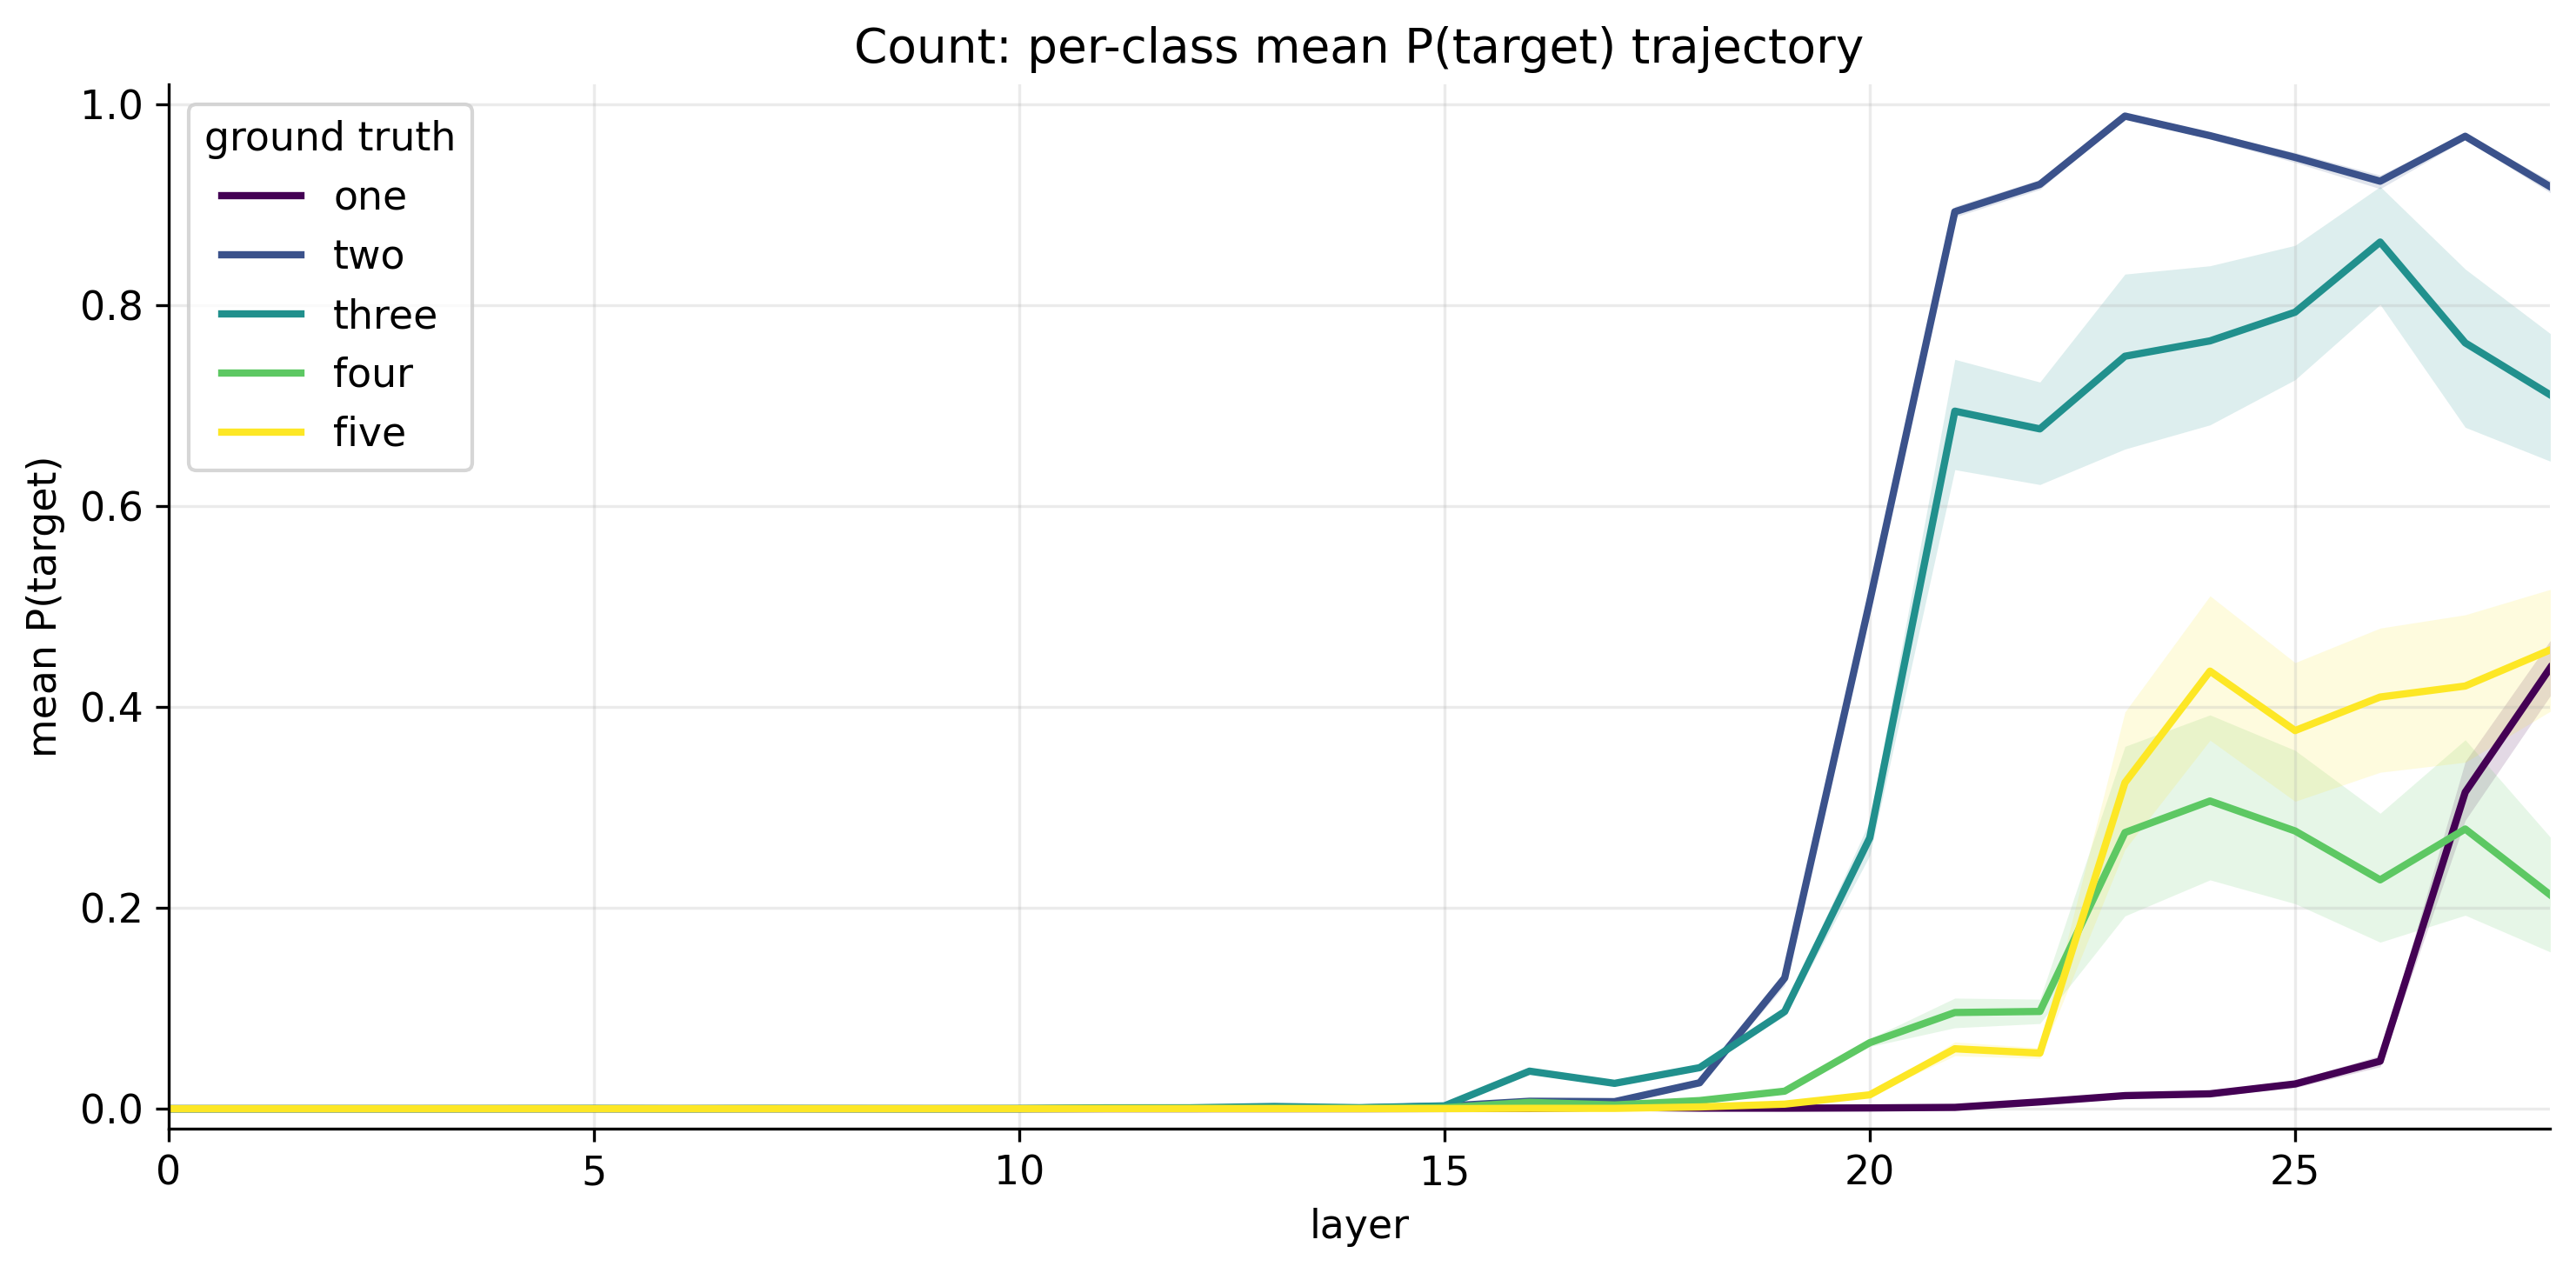
\includegraphics[width=\columnwidth]{fig5_count_breakdown.png}
    \caption{Count per-class trajectories. ``Two'' and ``three'' saturate by L21. ``Four'' and ``five'' plateau at 0.2--0.45. ``One'' only appears at L27.}
    \label{fig:count}
\end{figure}

Two distinct failure modes:

\paragraph{$n=4$ hard-floors at ``three.''}
Of the 39 wrong predictions on $n{=}4$ images, every single one is ``three.''
Not noise---a deterministic preference.
On $n{=}5$, 82\% of errors are ``four'' and the rest ``three,'' which looks like a one-step undercount baked in.

\paragraph{$n=1$ loses to a language prior.}
Count ``one'' emerges only at L27, vs.\ L19 for ``two''---which is jarring if you expect ``one'' to be the easy case.
The ``There are'' prefill biases toward plural continuation, so for L19 through L26 the model is voting ``two'' or ``three'' even on single-object images.
The visual evidence eventually wins, but only at the very last layer.
That's eight layers of language-vision tug-of-war.

L28 per-class accuracy: 1$\to$86\%, 2$\to$100\%, 3$\to$82\%, 4$\to$22\%, 5$\to$66\%.

\subsection{Spatial: The ``Below'' Blind Spot}

Three of four spatial relations work---left, right, and above all hit 100\% at L28.
``Below'' is broken: 10\% accuracy with all 45 errors producing ``right'' (\Cref{fig:spatial}).

\begin{figure}[t]
    \centering
    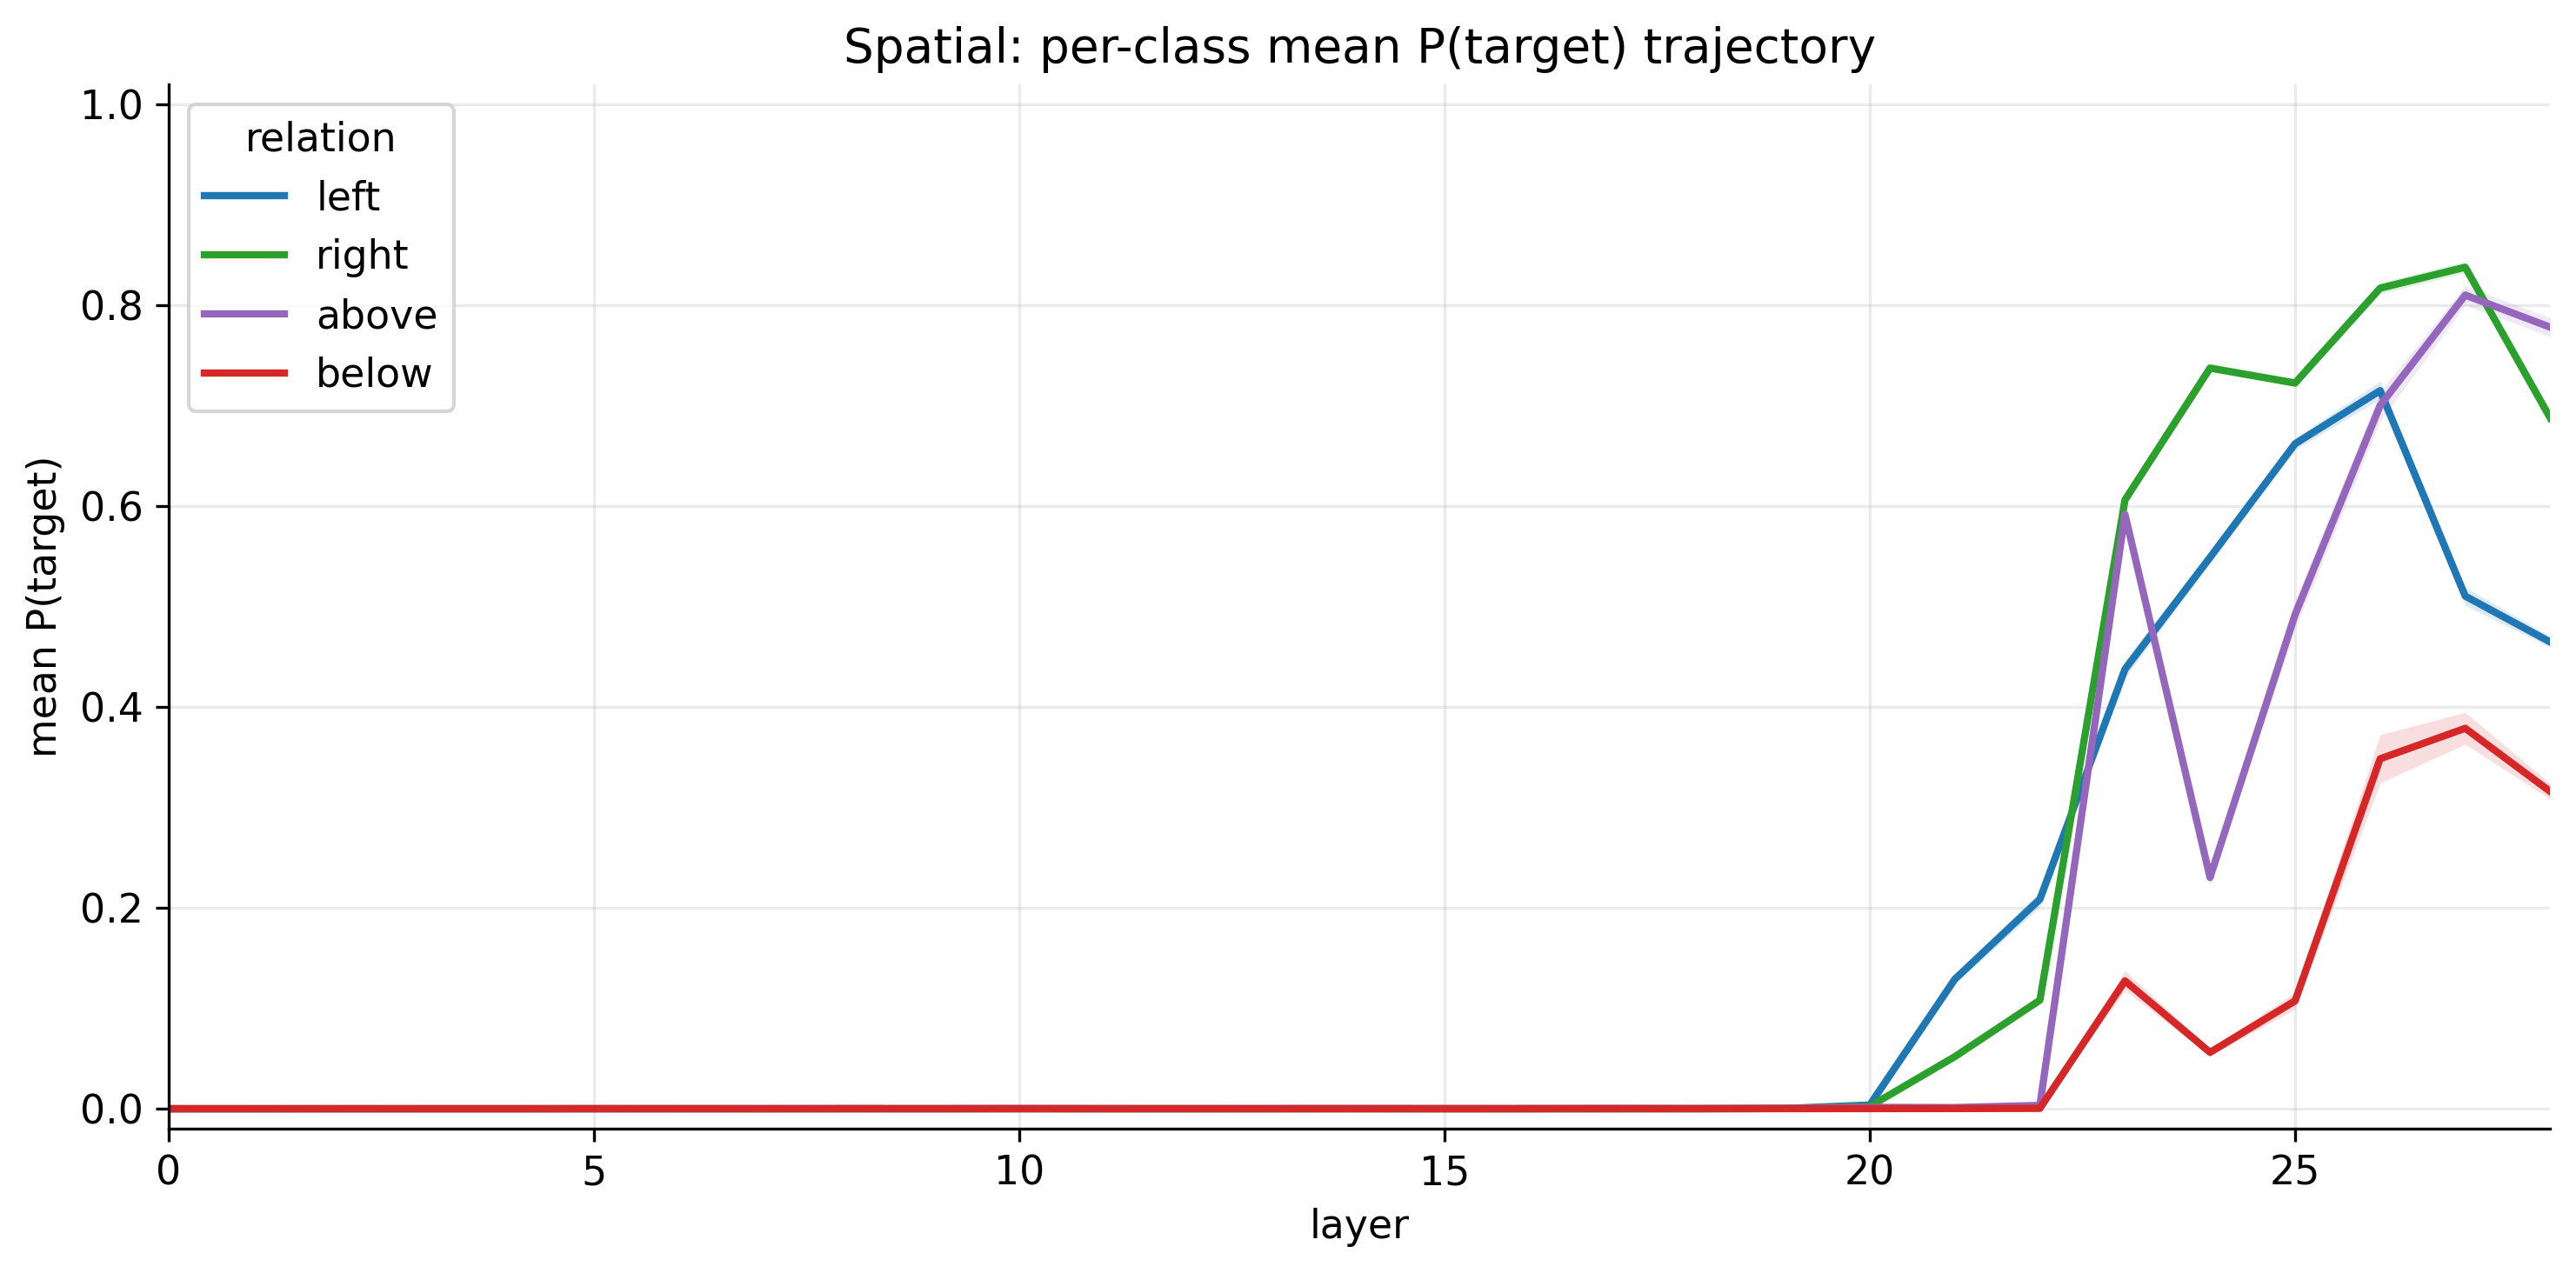
\includegraphics[width=\columnwidth]{fig6_spatial_breakdown.png}
    \caption{Spatial per-class trajectories. Left, right, and above climb out of zero at L21--L23. ``Below'' rises briefly at L23--L24, then \emph{actively decays}---late layers suppress the correct answer.}
    \label{fig:spatial}
\end{figure}

The trajectory is the strange part.
P(below) actually \emph{rises} at L23--L24, then drops back through L28---the model has partial information about ``below'' at mid-depth and the late layers overwrite it with ``right.''
That is not absence of a feature; it is active suppression by something.
I tried six prompt templates and an axis-aligned dataset redesign (zero perpendicular offset between objects), and got the same below$\to$right collapse every time, matching the ``weak spatial reasoning'' line on Qwen2-VL's own model card.

The working spatial classes are also globally weaker than color/shape---L28 P(target) is 0.47--0.78 here vs.\ 0.92--0.95 for the cleaner features---so spatial reasoning looks coarsely encoded across the board, not just on ``below.''

% ===================================================================
\section{Key Statements}
\label{sec:statements}

\textbf{Statement 1: Color and shape emerge in a sharp 2-layer phase transition at L22$\to$L23.}
P(target color) goes from 0.001 at L22 to 0.413 [0.391, 0.437] at L23; shape from 0.019 to 0.374 [0.337, 0.408].
By L25 the target is rank-0 in every image.
The whole transition lives in the last quarter of a 28-layer model---matching the L25/28 best-decoding layer that \citet{neo2025interpreting} report on the same backbone.

\textbf{Statement 2: Binding is compositional on this dataset---pair accuracy crosses 50\% at L24 and saturates at 100\%.}
Across 200 image pairs, P(distractor) never tops 0.01 and the L24 margin is +0.676 [0.665, 0.689].
The model knows which object the question is about as soon as it has anything to say---there is no ``both colors are likely'' midstream.

\textbf{Statement 3 (non-working): Counting collapses at $n \ge 4$---the model floors at ``three.''}
P(four) at L28 on $n{=}4$ images is 0.213 [0.159, 0.271], while P(two) on $n{=}2$ reaches 0.918 [0.912, 0.924].
``Four'' and ``five'' plateau after L23 and don't recover at any later depth.
That looks like a capacity ceiling rather than an optimization problem---the answer never appears in the residual stream.

\textbf{Statement 4 (non-working): ``Below'' is actively suppressed in late layers.}
P(below) at L28 is 0.316; accuracy 10\%; all 45 errors produce ``right.''
P(below) \emph{rises} through L24 and then decays---late layers overwrite a partially formed spatial answer with a directional prior.
Six prompt templates produce the same collapse, so this is a model-level blind spot, not a prompt artifact.

% ===================================================================
\section{Limitations}
\label{sec:limitations}

\textbf{Synthetic data.}
Solid shapes on flat gray backgrounds are very far OOD from this model's pretraining mix.
Real images would probably give smoother trajectories, possibly at different layers.

\textbf{Correlational, not causal.}
The lens shows that a feature is \emph{decodable} at layer $\ell$, not that the model \emph{uses} it there.
To claim use you need patching or ablation.

\textbf{Binding dataset is too clean.}
100\% pair accuracy and zero distractor probability come from a maximally easy setup---two well-separated objects, maximally distinct colors---not from a general VLM capability.
Natural-image binding fails routinely~\citep{yuksekgonul2023aro}.

% ===================================================================
\section{Conclusion}

Color, shape, and compositional binding all emerge sharply at L22--L23; counting breaks at $n\ge4$ and ``below'' gets overwritten in late layers.
The whole story plays out in the last quarter of the network---layers 0--21 produce no decodable visual signal.

% ===================================================================
\bibliography{references}
\bibliographystyle{icml2025}

\end{document}
